\chapter{Experimentation}
\label{sec:Experimentation}

The intuition behind developing a CNN on this dataset is novel. Many related works demonstrate the feasibility of using CNN models to classify or segment SAR imaging \cite{SAR-U-Net}, but tend not to explore regression tasks. This could be the result of a publicly unavailable dataset like the one derived in from the data collection. Furthermore, attempting to relate IS-2 footprints to high resolution SAR imaging involves deriving information from single-channel imagery of low pixel dimension. Compounded with the 33$\%$ yield of anticipated data from the ICEYE image, the limited data is exacerbated. With the different goal of this task and the limitations imposed upon it, it's apparent that the experimentation should draw from the findings and intuition of task-adjacent works.

To begin, the coincident data was extracted from the ICEYE imagery, yielding 4,683 17x17 tiles with associated LiDAR measurements. The selected densities used for interpolation as follows, where the snow density is drawn from historical measurements during the month of January \cite{warren1999snow}.

\begin{figure}[h]
  \[
  \begin{aligned}[t]
    \rho_i &=  \text{Density of sea ice }(916 \frac{kg}{m^3}) \\   %	It'd be perfect to place the diagram of the sheet in the white space generated here in latex
    \rho_s &=  \text{Density of snow }(300 \frac{kg}{m^3}) \\   %	It'd be perfect to place the diagram of the sheet in the white space generated here in latex
    \rho_w &=  \text{Density of water }(1024 \frac{kg}{m^3}) \\   %	It'd be perfect to place the diagram of the sheet in the white space generated here in latex
  \end{aligned}
\]
\end{figure}
  
Using Equation 1.1, each tile's elevation readings are converted to the associated thickness. Some values of freeboard were negative, and interpreted to mean there was no present snow and that the estimated sea ice height should be reduced to accommodate for the negative value. Each tile's interpolated ice thickness can be visualized in Figure 3.1.

\begin{figure}[h!]
	\centering
	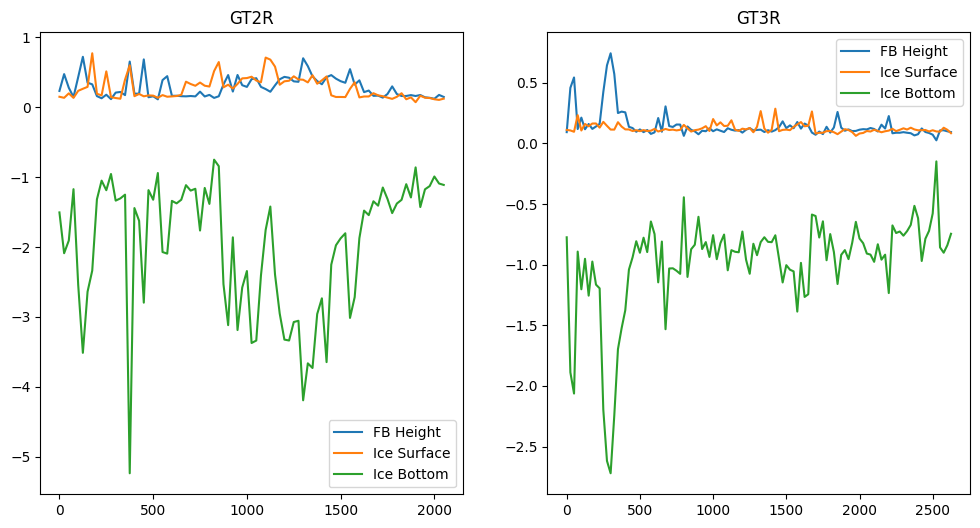
\includegraphics[width=\textwidth]{../research-resources/ice-sat-2/coincident-ice-profile.png}
	\caption{Interpolated Ice Thickness}
	\label{fig:ice-thickness-interpolation}
\end{figure}

\section {Feed Forward}

\cite{BASHA2020112}
\cite{jernelv2020convolutional}

\section {U-Net}